%METHODE DES CENTRES MOBILES (CM)

\subsubsection{Démarche}

La démarche pour les deux méthodes consiste à appliquer respectivement une ACP, après normalisation, et une ACM aux données, après mise en classe, puis de classer les résultats par une méthode des centres mobiles.

Les données utilisées dans l'exemple donné en graphique sont issues de la base "populations".

Ces données étant quantitatives, l'ACP peut s'appliquer directement, mais il faut réaliser une mise en classe pour obtenir un tableau disjonctif complet et réaliser l'ACM.

Une fois ces méthodes de factorisation appliquées, on peut appeler la fonction \textit{kmeans2} issue du module \textit{scipy.cluster.vq (K-means clustering and vector quantization)} pour réaliser une classification par la méthode des centres mobiles.

Dans les exemples de résultats ci-dessous, on a choisi respectivement un nombre de classes $k = 3$ et $5$ pour l'ACM et l'ACP arbitrairement en fonction du nombre de données pour obtenir des graphiques visibles tout en observant l'efficacité de la méthode.

Les étoiles représentent les centres, et les couleurs l'appartenance à la classe de chaque point.

    \begin{figure}[!htb]
        %\captionsetup[subfigure]{labelformat=empty}
        \begin{subfigure}[b]{0.48\textwidth}
            \centering
            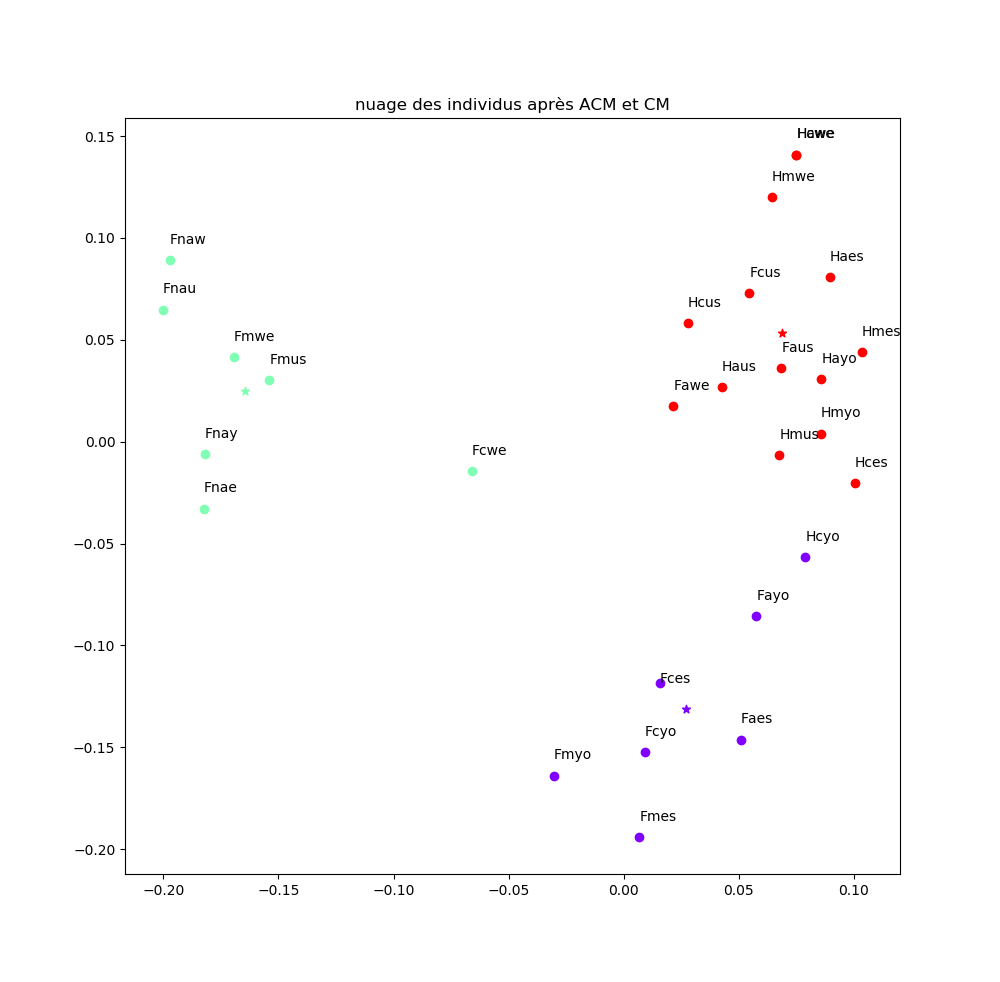
\includegraphics[width=0.98\textwidth]{img/Individus_ACM-CM.png}
            \caption{ACM + CM : Projection des individus}
            \label{Label_Individus_ACM-CM.png}
        \end{subfigure}
        \begin{subfigure}[b]{0.48\textwidth}
            \centering
            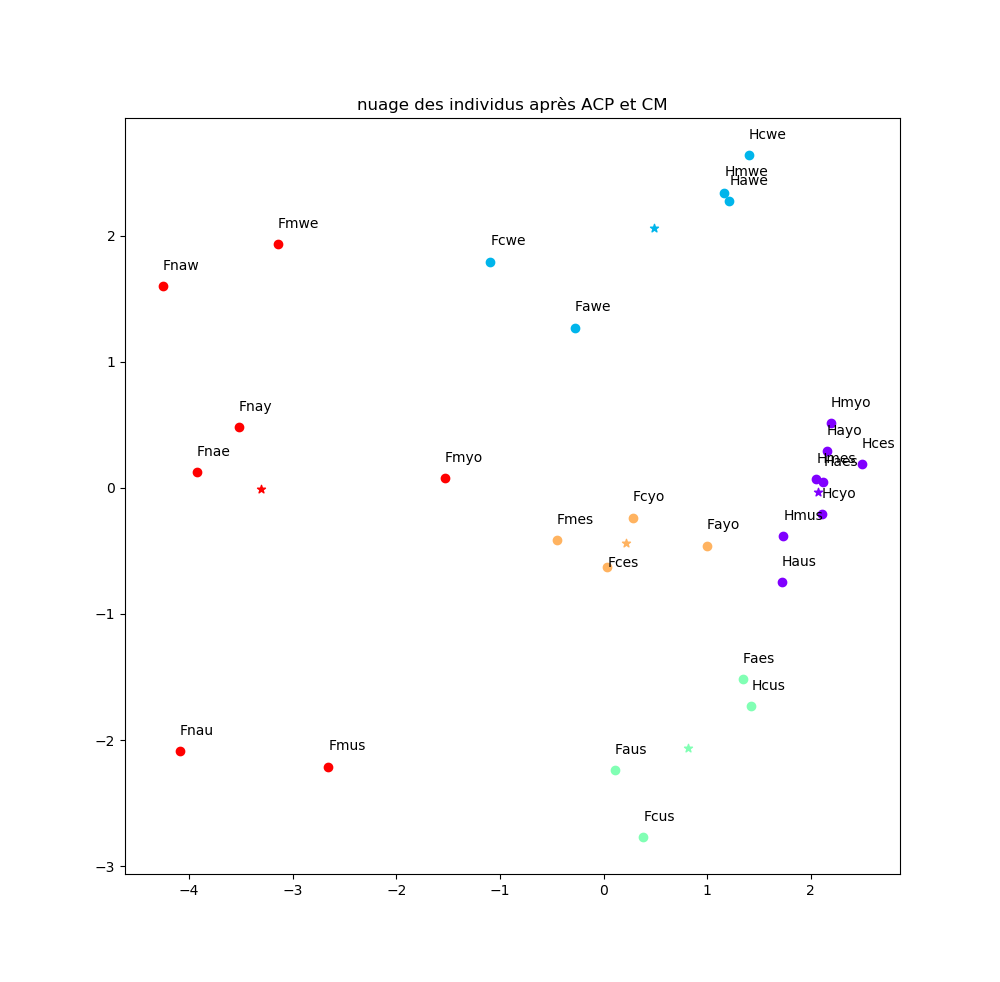
\includegraphics[width=0.98\textwidth]{img/Individus_ACP-CM.png}
            \caption{ACP + CM : Projection des individus}
            \label{Label_Individus_ACP-CM.png}
        \end{subfigure}
        \caption{Résultats pour l'ACP/ACM + CM : Projection des individus}
        \label{Label_Individus_ACP_ACM-CM.png}
    \end{figure}
    
    \begin{figure}[!htb]
        %\captionsetup[subfigure]{labelformat=empty}
        \begin{subfigure}[b]{0.48\textwidth}
            \centering
            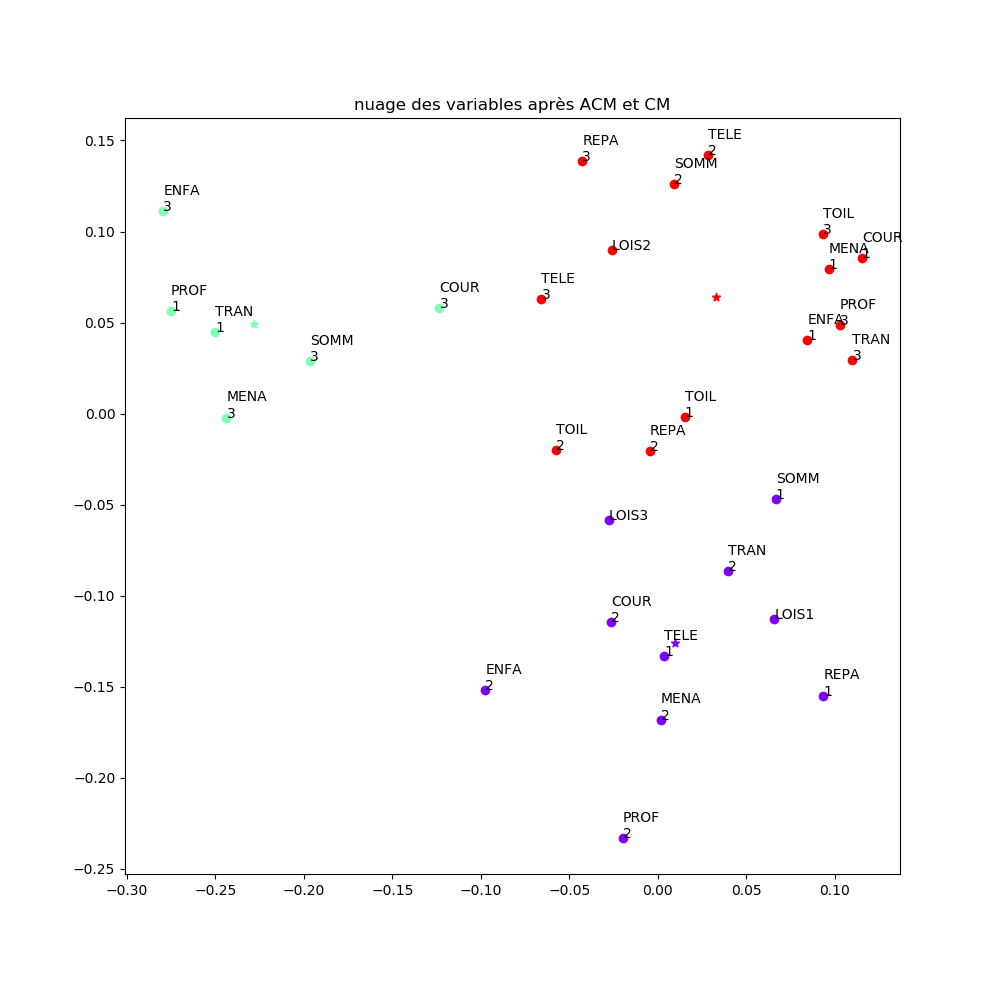
\includegraphics[width=0.98\textwidth]{img/Variables_ACM-CM.png}
            \caption{ACM + CM : Projection des variables}
            \label{Label_Variables_ACM-CM.png}
        \end{subfigure}
        \begin{subfigure}[b]{0.48\textwidth}
            \centering
            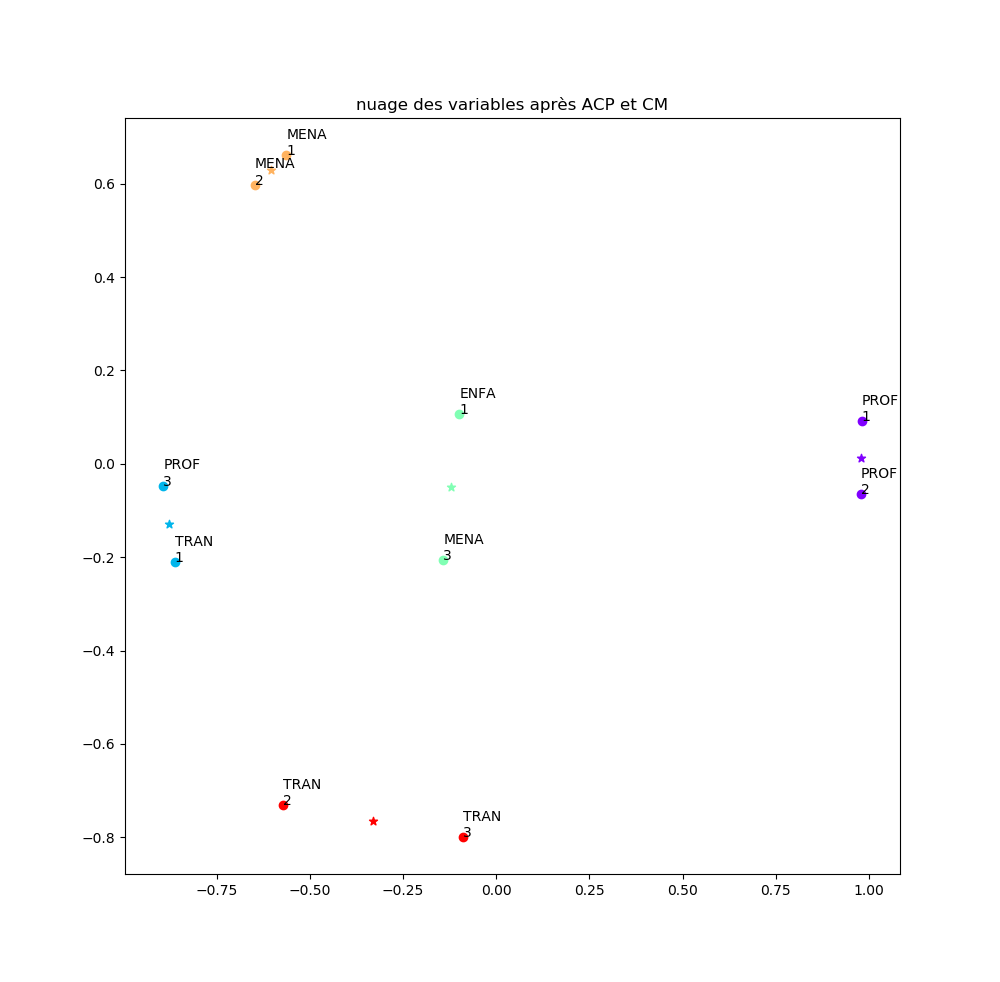
\includegraphics[width=0.98\textwidth]{img/Variables_ACP-CM.png}
            \caption{ACP + CM : Projection des variables}
            \label{Label_Variables_ACP-CM.png}
        \end{subfigure}
        \caption{Résultats pour l'ACP/ACM + CM : Projection des variables}
        \label{Label_Variables_ACP_ACM-CM.png}
    \end{figure}
    
\subsubsection{Commentaires et interprétation}


On a observé ci dessus une classification satisfaisante des éléments, sans points aberrants. Cela permet dans l'exemple de données traité, de regrouper les métiers et occupations des individus en fonction du temps que cela leur prend, par exemple.

On peut néanmoins observer en appliquant plusieurs fois la méthodes, que la fonction place parfois un (ou plusieurs) centre isolé, ce qui rend une classe entière obsolète (cf. Figure \ref{fig: Label Classes_obsoletes_ACP-CM.png}.

%------ Pour insérer et citer une image centralisée -----
\insererfigure{img/Classes_obsoletes_ACP-CM.png}{14 cm}{Cas des centres isolés}{Label Classes_obsoletes_ACP-CM.png}
% Le premier argument est le chemin pour la photo
% Le deuxième est la hauteur de la photo
% Le troisième la légende
% Le quatrième le label)

Dans l'exemple de résultat pour l'ACP ci-dessous, deux centres sur cinq ont été mal placés dans la représentation du nuage des individus. Il est à noter que cela n'implique pas un mauvais placement pour le nuage des variables. Cela montre une limitation de la méthode des centres mobiles, qui présente, due à son caractère aléatoire de placement de centres, des résultats parfois non conformes aux consignes, et nuisant à la bonne interprétation des données.

